% !TEX root = main.tex
\section{数値実験}

\subsection{課題 1}
\subsubsection{課題内容}
最適化アルゴリズムの評価には,さまざまなテスト関数が利用されている.\textbf{Rastrigin 関数以外}の単一目的関数を調査し,それらの特徴を整理して Python で実装しなさい.

文献\cite{ref4}などを参考にし,最適化アルゴリズムのベンチマーク関数としてよく使用されるテスト関数について調査する.

なお,テスト関数の性質としては以下のような要素がある.

\begin{itemize}
  \item \textbf{単峰性関数(Unimodal functions)}:最適解がただ一つの谷に存在する関数
  \item \textbf{多峰性関数(Multimodal functions)}:最適解が複数の谷に存在する関数
  \item \textbf{変数間の依存関係の有無(Variable dependencies)}:変数が独立しているか,または相互に依存しているか
\end{itemize}

具体的なテスト関数として,次に示す3つの関数を紹介する.これらの関数は最適化問題において広く利用され,それぞれ異なる性質を持っている.

\begin{itemize}
  \item \textbf{Sphere 関数}:この関数は,すべての変数が独立しており,最適解は原点(全ての変数が 0)にある.
  \[
    f_{\mathrm{Sphere}}(x_i) = \sum_{i=1}^{D} x_i^2,\quad (-10 \leq x_i \leq 10) \tag{6}
  \]

  \item \textbf{Rosenbrock 関数(Rosenbrock-Star)}:この関数は,変数間に依存関係がある.
  \[
    f_{\mathrm{Rosenbrock\mbox{-}Star}}(x_i) = \sum_{i=1}^{D-1} \left\{100(x_{i+1} - x_i^2)^2 + (x_i - 1.0)^2 \right\},\quad (-10 \leq x_i \leq 10) \tag{7}
  \]

  \item \textbf{Griewank 関数}:この関数は,複数の変数が相互に影響し合う形式で,非常に多くの局所最小値を持っている.
  \[
    f_{\mathrm{Griewank}}(x_i) = \frac{1}{4000} \sum_{i=1}^{n} x_i^2 - \prod_{i=1}^{n} \cos\left(\frac{x_i}{\sqrt{i}}\right) + 1,\quad (-500 \leq x_i \leq 500) \tag{8}
  \]
\end{itemize}

各関数の特徴を理解し,それぞれ Python で実装する.そして,実装したテスト関数を利用し,PSO で最適化を行いなさい.
\subsubsection{課題結果及び考察}
本課題では,PSO(Particle Swarm Optimization)アルゴリズムを用いて,代表的な4種類のベンチマーク関数
(Sphere関数,Rosenbrock関数,Griewank関数,Rastrigin関数)の最小値探索を行い,それぞれの関数に対するPSOの収束特性を比較した.

図\ref{fig:convergence}に,各関数に対する最良評価値の世代ごとの推移を示す.
この図から,関数ごとの最適化難易度やPSOの探索性能に対する関数特性の影響を明確に観察することができた.

まず,\textbf{Sphere関数}においては,最も単純な単峰性かつ変数独立型の関数であり,PSOは初期世代から非常に滑らかに最適解へと収束している.
この関数では,全変数が原点を最小値とするため,PSOのグローバル探索能力が十分に発揮され,収束速度も極めて高速であった.

一方,\textbf{Rosenbrock関数}では,変数間に強い依存関係が存在し,評価関数の谷が非常に細く曲がっているため,PSOにとっては難易度の高い最適化問題である.
実験結果においても,初期段階で評価値が非常に高く,収束に時間を要していることが確認された.ただし,世代が進むにつれて評価値は着実に改善されており,
PSOが谷に沿って最適解に近づいていく様子が伺える.

次に,\textbf{Griewank関数}と\textbf{Rastrigin関数}は多峰性の関数であり,多数の局所最小値が存在する.
しかし,Griewank関数は4つの関数な中で一番早く収束している.一方で,Rastrigin関数は,Griewank関数よりも収束がやや遅くなっていることが観察された.
それでもPSOはこれらの局所解に捕まることなく,目的関数値を徐々に改善しており,多峰性関数に対しても有効な探索能力を示した.

以上の結果から,PSOは単純な関数に対しては非常に高い収束性能を示し,多峰性関数においても一定の効果を発揮することが確認できた.

\begin{figure}[H]
    \centering
    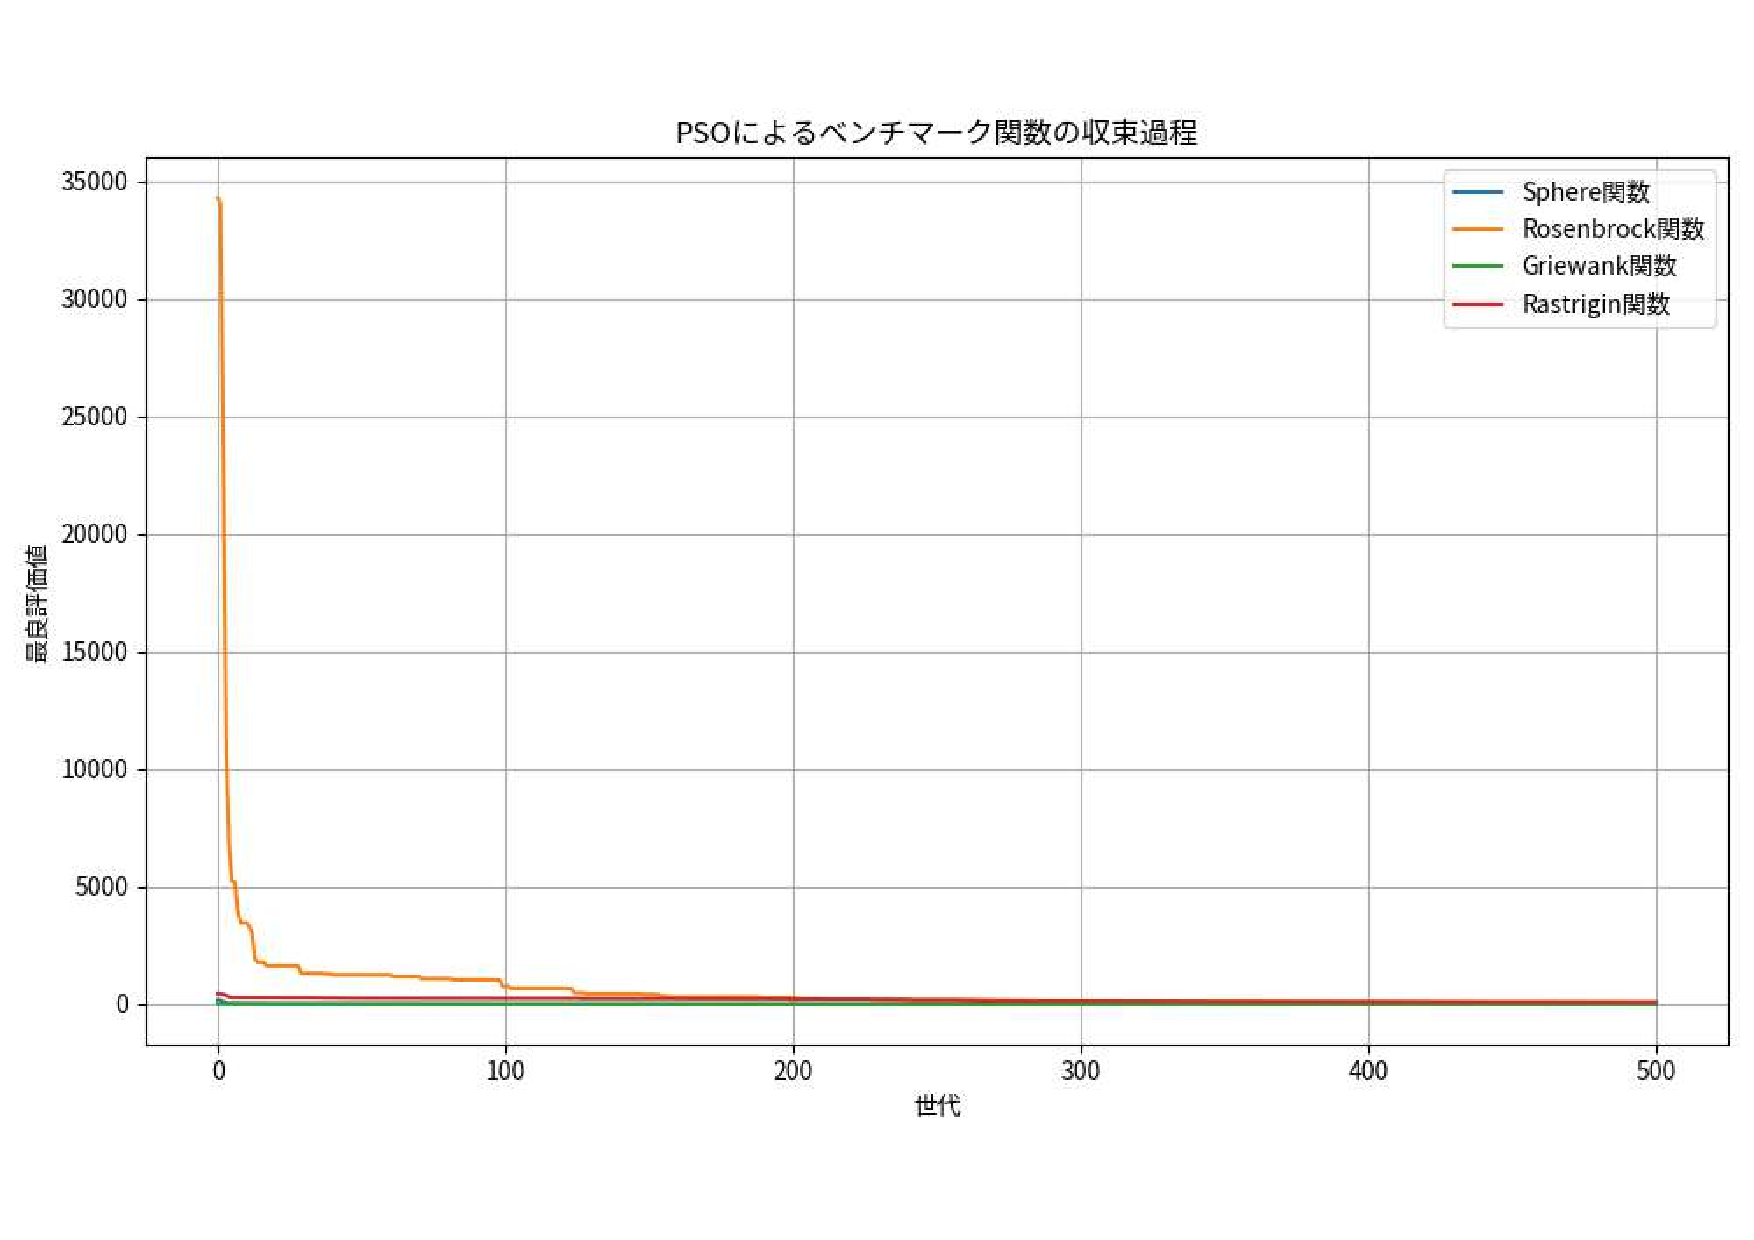
\includegraphics[width=0.8\linewidth]{figure/収束グラフ.pdf}
    \caption{PSOによるベンチマーク関数の収束過程}
    \label{fig:convergence}
\end{figure}

\begin{figure}[H]
    \centering
    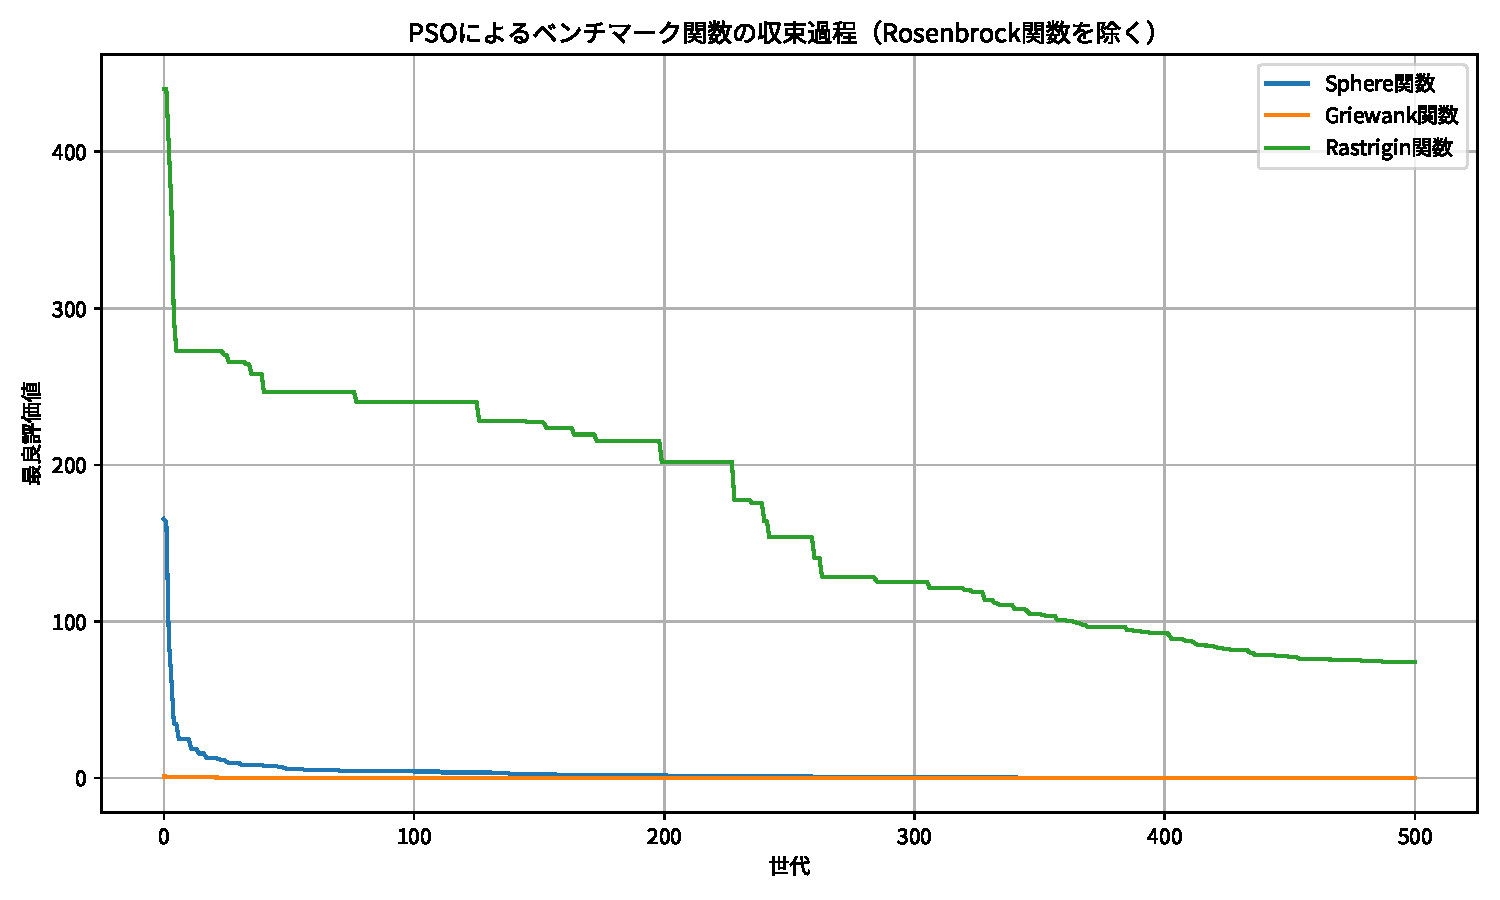
\includegraphics[width=0.8\linewidth]{figure/Figure_1.pdf}
    \caption{PSOによるベンチマーク関数の収束過程(Rosenbrock関数を除く)}
    \label{fig:convergence2}
\end{figure}


\newpage
\subsubsection{使用したプログラムコード}

\begin{lstlisting}[caption=PSOによるベンチマーク関数の最適化, label=lst:pso_code]
import os
import math
import random
import matplotlib.pyplot as plt
import pandas as pd

# 日本語フォント設定
plt.rcParams['font.family'] = 'Noto Sans CJK JP'

def fitFuncSphere(xVals):
    return sum(x**2 for x in xVals)

def fitFuncRosenbrock(xVals):
    return sum(100 * (xVals[i] - xVals[i-1])**2 + (xVals[i-1] - 1)**2 for i in range(1, len(xVals)))

def fitFuncGriewank(xVals):
    sum_term = sum(x**2 for x in xVals) / 4000
    prod_term = 1
    for i in range(len(xVals)):
        prod_term *= math.cos(xVals[i] / math.sqrt(i + 1))
    return sum_term - prod_term + 1

def fitFuncRastrigin(xVals):
    return 10 * len(xVals) + sum(x**2 - 10 * math.cos(2 * math.pi * x) for x in xVals)

def initPosition(Np, Nd, xMin, xMax):
    return [[xMin + random.random() * (xMax - xMin) for _ in range(Nd)] for _ in range(Np)]

def initVelocity(Np, Nd, vMin, vMax):
    return [[vMin + random.random() * (vMax - vMin) for _ in range(Nd)] for _ in range(Np)]

def updateVelocity(R, V, Np, Nd, j, w, vMin, vMax, pBestPos, gBestPos, c1, c2):
    for p in range(Np):
        for i in range(Nd):
            r1 = random.random()
            r2 = random.random()
            V[p][i] = (w * V[p][i] +
                       c1 * r1 * (pBestPos[p][i] - R[p][i]) +
                       c2 * r2 * (gBestPos[i] - R[p][i]))
            V[p][i] = max(min(V[p][i], vMax), vMin)

def updatePosition(R, V, Np, Nd, xMin, xMax):
    for p in range(Np):
        for i in range(Nd):
            R[p][i] += V[p][i]
            R[p][i] = max(min(R[p][i], xMax), xMin)

def updateFitness(R, M, Np, pBestPos, pBestVal, gBestPos, gBestValue, fitFunc):
    for p in range(Np):
        M[p] = fitFunc(R[p])
        if M[p] < gBestValue:
            gBestValue = M[p]
            gBestPos[:] = R[p][:]
        if M[p] < pBestVal[p]:
            pBestVal[p] = M[p]
            pBestPos[p][:] = R[p][:]
    return gBestValue

def runPSO(fitFunc, name, Np=30, Nd=30, Nt=500,
           xMin=-5.12, xMax=5.12,
           vMin=None, vMax=None,
           wMin=0.4, wMax=0.9, c1=2.05, c2=2.05):

    vMin = vMin if vMin is not None else 0.25 * xMin
    vMax = vMax if vMax is not None else 0.25 * xMax

    R = initPosition(Np, Nd, xMin, xMax)
    V = initVelocity(Np, Nd, vMin, vMax)
    M = [fitFunc(R[p]) for p in range(Np)]
    pBestVal = M[:]
    pBestPos = [r[:] for r in R]
    gBestValue = min(M)
    gBestPos = R[M.index(gBestValue)][:]
    history = [gBestValue]

    for j in range(Nt):
        w = wMax - (wMax - wMin) * j / Nt
        updatePosition(R, V, Np, Nd, xMin, xMax)
        gBestValue = updateFitness(R, M, Np, pBestPos, pBestVal, gBestPos, gBestValue, fitFunc)
        updateVelocity(R, V, Np, Nd, j, w, vMin, vMax, pBestPos, gBestPos, c1, c2)
        history.append(gBestValue)
    
    return name, history

def main():
    output_dir = "./実験1結果"
    os.makedirs(output_dir, exist_ok=True)

    benchmark_funcs = [
        (fitFuncSphere, "Sphere関数"),
        (fitFuncRosenbrock, "Rosenbrock関数"),
        (fitFuncGriewank, "Griewank関数"),
        (fitFuncRastrigin, "Rastrigin関数")
    ]

    all_histories = []
    df_data = {}

    for func, name in benchmark_funcs:
        print(f"{name} のPSO最適化を実行中...")
        name, history = runPSO(func, name)
        all_histories.append((name, history))
        df_data[name] = history

    df = pd.DataFrame(df_data)
    df.index.name = "世代"
    df.to_csv(os.path.join(output_dir, "収束履歴表.csv"))

    plt.figure(figsize=(10, 6))
    for name, history in all_histories:
        plt.plot(history, label=name)
    plt.xlabel("世代")
    plt.ylabel("最良評価値")
    plt.title("PSOによるベンチマーク関数の収束過程")
    plt.legend()
    plt.grid(True)
    plt.tight_layout()
    plt.savefig("figure/収束グラフ.pdf")
    plt.show()

if __name__ == "__main__":
    main()
\end{lstlisting}

%%%%%%%%%%%%%%%%%%%%%%%%%%%%%%%%%%%%%%%%%%%%%%%%%%%%%%%%%%%%%%%%%%%%%%%%%%%%%%%%%%%%%%%%%%%%%%%%%%%%%%%%%%%%%%%%%%%%%%%%%%
\subsection{課題 2}

\subsubsection{課題内容}
本課題では,PSO(Particle Swarm Optimization)における各種パラメータが最適化性能に与える影響について数値実験を通して検証する.
評価関数として多峰性かつ非線形な難関関数であるRastrigin関数を用い,以下の5種類の条件で比較実験を行う.
\begin{table}[H]
    \centering
    \caption{PSOにおける各パラメータ設定}
    \label{tab:pso_param}
    \begin{tabular}{lccc}
      \hline
      設定名 & $c_1 = c_2$ & $w_{\mathrm{max}}$ & $w_{\mathrm{min}}$ \\
      \hline
      Standard(標準) & 2.05 & 0.75 & 0.40 \\
      Low\_acc(加速度係数小) & 1.00 & 0.75 & 0.40 \\
      High\_acc(加速度係数大) & 3.00 & 0.75 & 0.40 \\
      High\_inertia(慣性項大) & 2.05 & 0.90 & 0.65 \\
      Low\_inertia(慣性項小) & 2.05 & 0.60 & 0.30 \\
      \hline
    \end{tabular}
  \end{table}
各設定の詳細は表\ref{tab:pso_param}に示す通りである.  
他のパラメータはすべて以下に統一し,10回の試行平均により評価した.

\begin{itemize}
  \item 粒子数 \(Np = 20\)
  \item 次元数 \(Nd = 20\)
  \item 繰り返し回数 \(Nt = 1000\)
  \item 定義域 \([-500, 500]\)
\end{itemize}

\subsubsection{課題結果および考察}
図\ref{fig:kadai2_comparison}は,各設定におけるPSOの最良適応度の収束過程を比較したものである.

まず,\textbf{Standard}設定では滑らかに収束しており,PSOの代表的な挙動として安定した性能を発揮している.これを基準として,他の設定と比較する.

\textbf{Low\_acc}(加速度係数小)の結果では,探索範囲が狭まり,局所解からの脱出能力が弱まったため,早期に収束はするが精度の高い解に至りにくい傾向が見られた.

一方,\textbf{High\_acc}(加速度係数大)の結果では,大きなジャンプを伴うため初期の探索は広域に及ぶが,解に対して収束が遅くなる傾向があった.後半でも評価値の改善が遅く,収束性がやや劣る結果となった.

\textbf{High\_inertia}(慣性項大)は,過去の速度成分をより多く反映するため,探索範囲の拡張に寄与し,全体的に高い精度に到達する傾向が見られた.

これに対して,\textbf{Low\_inertia}(慣性項小)は,過去の移動履歴を無視するため,探索が局所的になりやすく,最適解に至らずに収束してしまうケースが多かった.

総じて,パラメータ設定はPSOの探索能力に大きな影響を与えることが確認された.特に加速度係数や慣性項は,探索の局所性とグローバル性のバランスに関与するため,適切な設定が必要である.今回の実験では,標準設定が最も安定した性能を示し,汎用的な選択肢として有効であることが示唆された.

\begin{figure}[H]
    \centering
    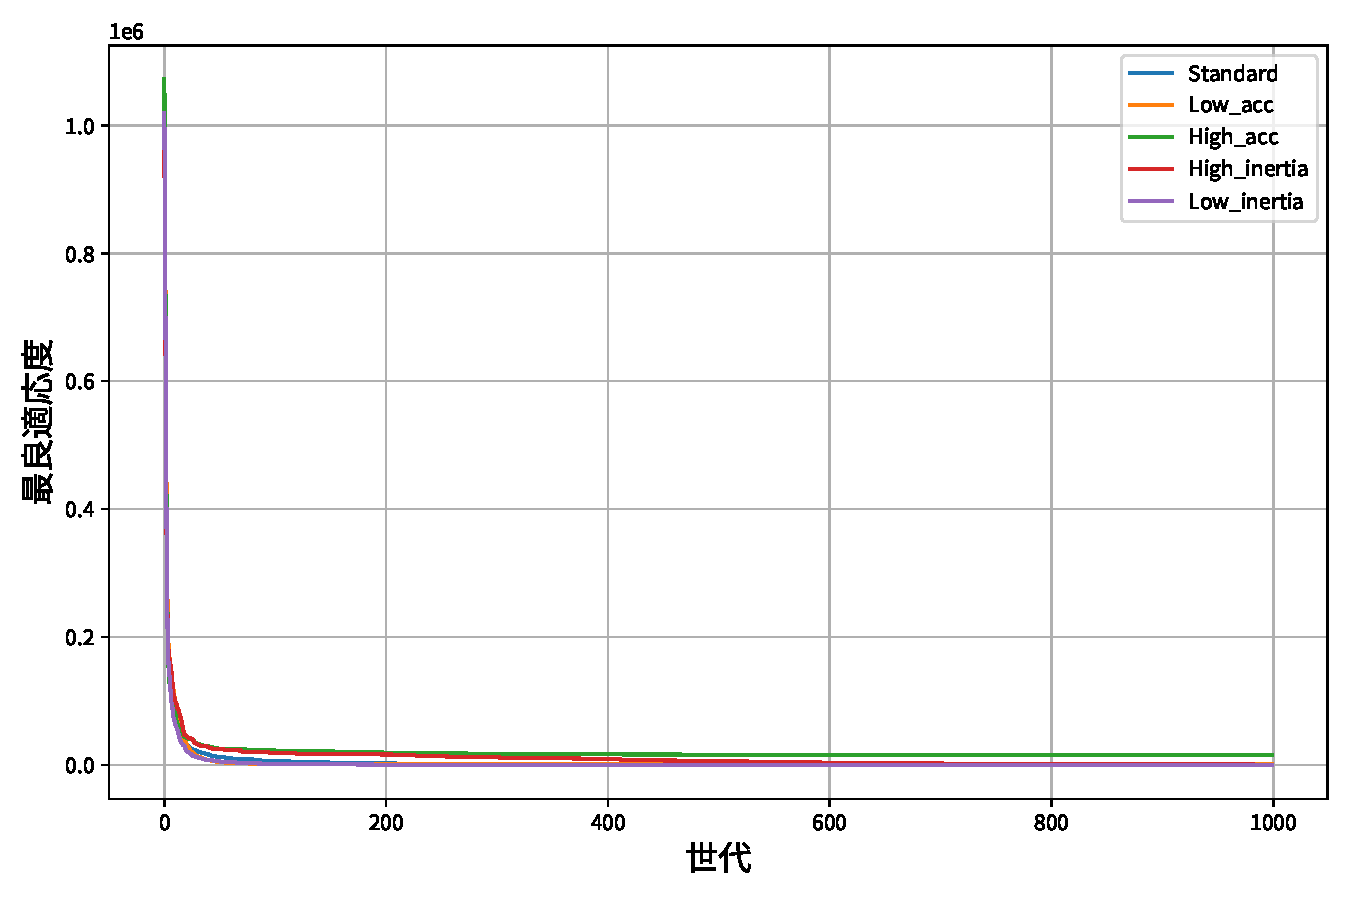
\includegraphics[width=0.9\linewidth]{figure/kadai2_comparison_graph.pdf}
    \caption{PSOにおける各パラメータ設定の収束過程の比較}
    \label{fig:kadai2_comparison}
\end{figure}

\begin{figure}[H]
    \centering
    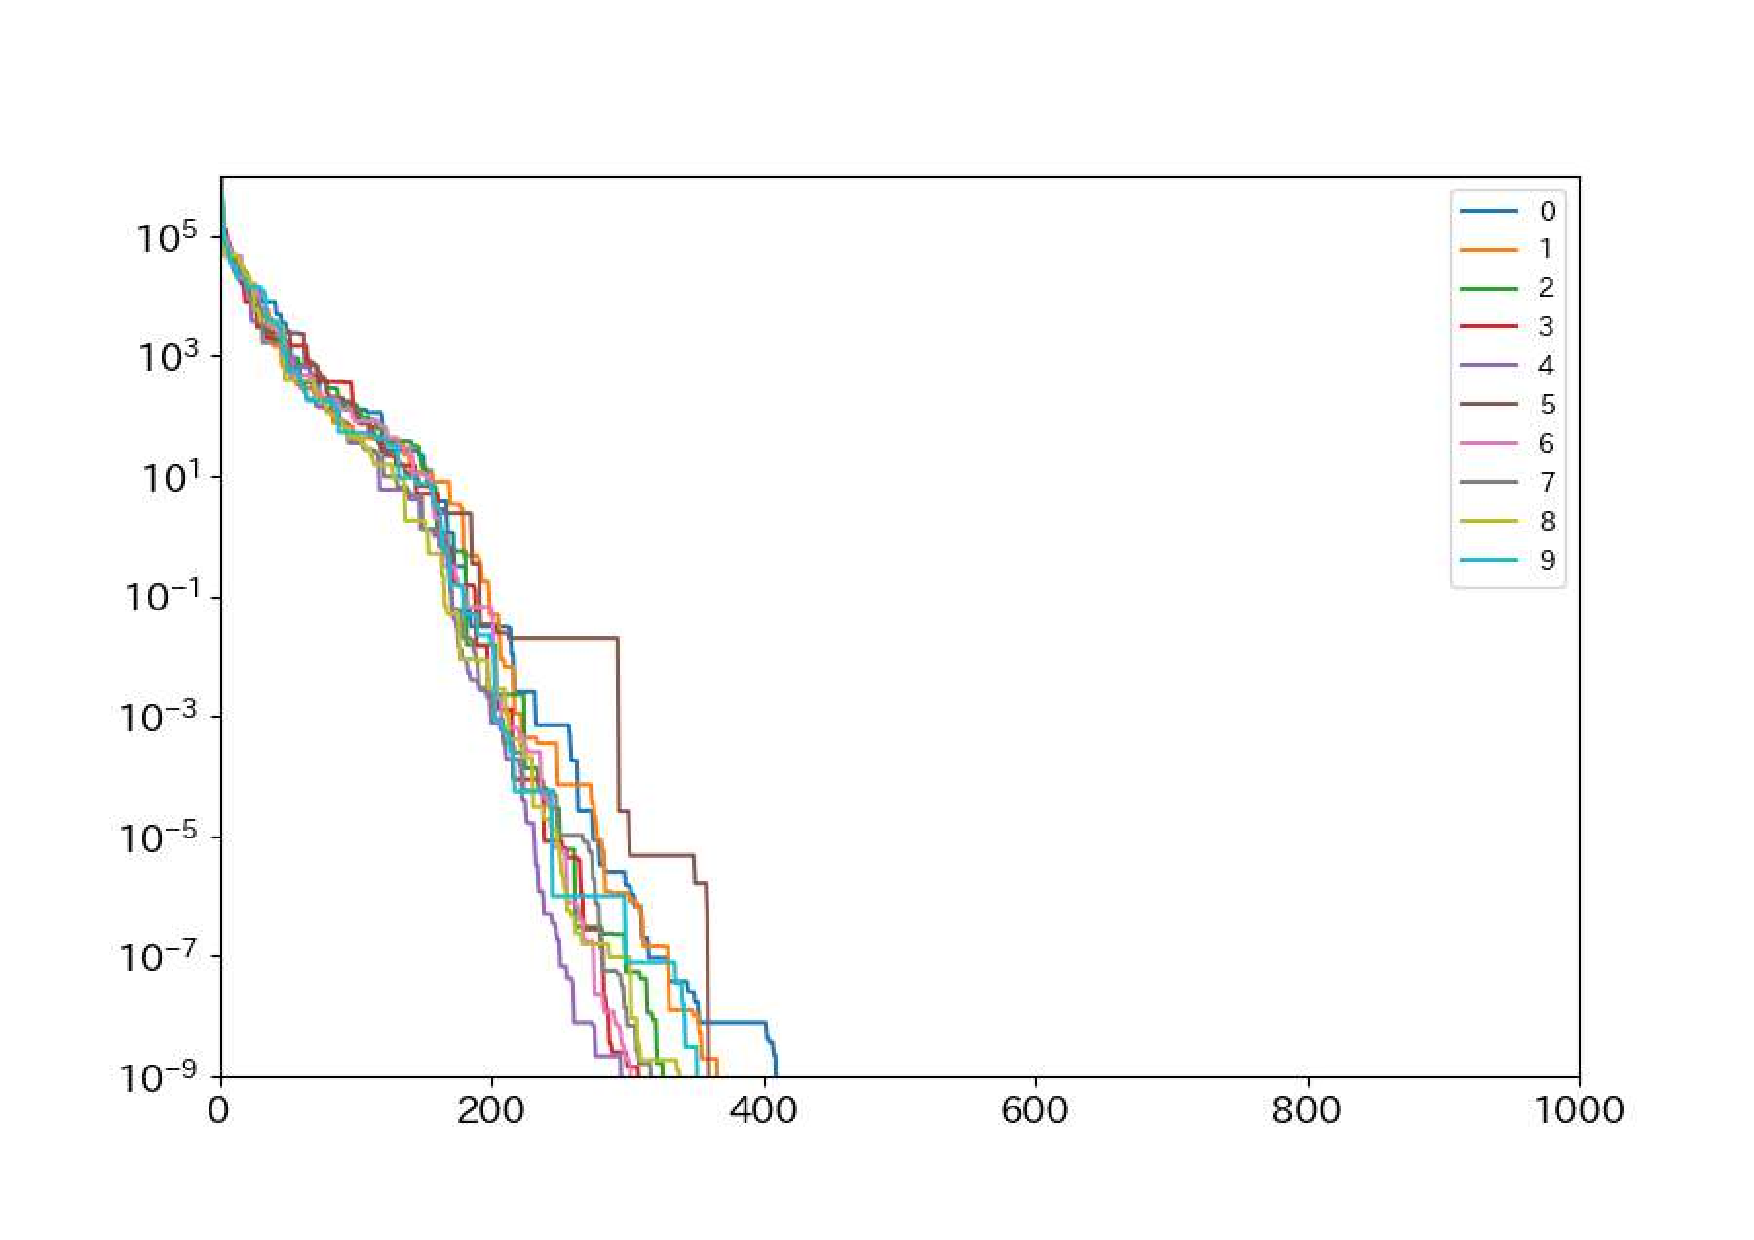
\includegraphics[width=0.9\linewidth]{figure/kadai2_result_graph_fixed.pdf}
    \caption{Rastrigin関数に対するPSO(標準パラメータ)の収束過程(10試行)}
    \label{fig:kadai2result}
\end{figure}

\newpage
\subsubsection{使用したプログラムコード}
\begin{lstlisting}[caption=PSOにおける各種パラメータ設定の比較実験コード, label=lst:kadai2_code]
    import os
    import math
    import random
    import numpy as np
    import pandas as pd
    import matplotlib.pyplot as plt
    
    # フォント設定(日本語表示)
    plt.rcParams['font.family'] = 'Noto Sans JP'
    # Rastrigin関数の定義
    def fitFunc1(xVals):
        fitness = 10 * len(xVals)
        for x in xVals:
            fitness += x**2 - 10 * math.cos(2 * math.pi * x)
        return fitness
    
    # 粒子の位置情報の初期化
    def initPosition(Np, Nd, xMin, xMax):
        return [[xMin + random.random() * (xMax - xMin) for _ in range(Nd)] for _ in range(Np)]
    
    # 粒子の速度情報の初期化
    def initVelocity(Np, Nd, vMin, vMax):
        return [[vMin + random.random() * (vMax - vMin) for _ in range(Nd)] for _ in range(Np)]
    
    # 粒子の位置ベクトルの更新
    def updatePosition(R, V, Np, Nd, xMin, xMax):
        for p in range(Np):
            for i in range(Nd):
                R[p][i] += V[p][i]
                R[p][i] = max(min(R[p][i], xMax), xMin)
    
    # 粒子の速度ベクトルの更新
    def updateVelocity(R, V, Np, Nd, j, w, vMin, vMax, pBestPos, gBestPos, c1, c2):
        for p in range(Np):
            for i in range(Nd):
                r1 = random.random()
                r2 = random.random()
                V[p][i] = (w * V[p][i] +
                           r1 * c1 * (pBestPos[p][i] - R[p][i]) +
                           r2 * c2 * (gBestPos[i] - R[p][i]))
                V[p][i] = max(min(V[p][i], vMax), vMin)
    
    # 粒子の評価値の更新
    def updateFitness(R, M, Np, pBestPos, pBestVal, gBestPos, gBestValue):
        for p in range(Np):
            M[p] = fitFunc1(R[p])
            if M[p] < gBestValue:
                gBestValue = M[p]
                gBestPos[:] = R[p][:]
            if M[p] < pBestVal[p]:
                pBestVal[p] = M[p]
                pBestPos[p][:] = R[p][:]
        return gBestValue
    
    def run_experiment(c1, c2, w_max, w_min, ITR=10):
        Np, Nd, Nt = 20, 20, 1000
        xMin, xMax = -500, 500
        vMin, vMax = 0.25 * xMin, 0.25 * xMax
        history_all = np.empty((ITR, Nt))
        for itr in range(ITR):
            R = initPosition(Np, Nd, xMin, xMax)
            V = initVelocity(Np, Nd, vMin, vMax)
            M = [fitFunc1(r) for r in R]
            pBestVal = M[:]
            pBestPos = [r[:] for r in R]
            gBestValue = min(M)
            gBestPos = R[M.index(gBestValue)][:]
            for j in range(Nt):
                updatePosition(R, V, Np, Nd, xMin, xMax)
                gBestValue = updateFitness(R, M, Np, pBestPos, pBestVal, gBestPos, gBestValue)
                # 線形減衰による慣性項の更新
                w = w_max - ((w_max - w_min) / Nt) * j
                updateVelocity(R, V, Np, Nd, j, w, vMin, vMax, pBestPos, gBestPos, c1, c2)
                history_all[itr][j] = gBestValue
        return np.mean(history_all, axis=0)
    
    def main():
        # 複数パラメータ設定による比較実験
        param_sets = {
            "Standard":    {"c1": 2.05, "c2": 2.05, "w_max": 0.75, "w_min": 0.4},
            "Low_acc":     {"c1": 1.0,  "c2": 1.0,  "w_max": 0.75, "w_min": 0.4},
            "High_acc":    {"c1": 3.0,  "c2": 3.0,  "w_max": 0.75, "w_min": 0.4},
            "High_inertia":{"c1": 2.05, "c2": 2.05, "w_max": 0.9,  "w_min": 0.65},
            "Low_inertia": {"c1": 2.05, "c2": 2.05, "w_max": 0.6,  "w_min": 0.3},
        }
        results = {}
        for key, params in param_sets.items():
            print(f"{key} パラメータで実験中...")
            results[key] = run_experiment(**params)
        
        output_dir = "実験2結果考察"
        os.makedirs(output_dir, exist_ok=True)
        df = pd.DataFrame(results)
        df.index.name = "世代"
        df.to_csv(os.path.join(output_dir, "kadai2_comparison_history.csv"))
        
        plt.figure(figsize=(9,6))
        for key, history in results.items():
            plt.plot(history, label=key)
        plt.xlabel("世代", size=16)
        plt.ylabel("最良適応度", size=16)
        plt.legend()
        plt.grid(True)
        plt.tight_layout()
        plt.savefig(os.path.join(output_dir, "kadai2_comparison_graph.png"))
        plt.show()
    
    if __name__ == "__main__":
        main()
\end{lstlisting}

%%%%%%%%%%%%%%%%%%%%%%%%%%%%%%%%%%%%%%%%%%%%%%%%%%%%%%%%%%%%%%%%%%%%%%%%%%%%%%%%%%%%%%


\subsection{課題3}
\subsubsection{課題内容}
課題1および課題2で得られた実験結果を基に,PSO(Particle Swarm Optimization)アルゴリズムが
「簡単な問題」と「難しい問題」に対して,
どのような収束特性を示すかについて考察を行う.

\subsubsection{課題結果および考察}
PSOアルゴリズムにおける探索性能は,対象とする最適化問題の性質に大きく影響されることが,課題1と課題2の実験結果から確認された.

まず,\textbf{Sphere関数}のような単峰性かつ変数間の依存関係がないシンプルな関数に対しては,PSOは非常に高い収束性能を示した.
評価値は初期世代から急激に減少し,短期間で最適解に到達した.このような関数では,局所解に迷い込むリスクがなく,PSOのグローバルな探索能力が最大限に発揮される.

一方で,\textbf{Rosenbrock関数}のように変数間に強い依存関係がある場合,評価関数の谷が細く曲がりくねっているため,
PSOは探索方向の調整に時間を要し,収束が遅くなる傾向が見られた.最適解への経路が単純ではないため,初期の探索では評価値がほとんど改善されない場合もあった.

また,\textbf{Rastrigin関数}や\textbf{Griewank関数}のように多峰性で局所最小値が多数存在する関数においては,
PSOは局所解に一時的に捕らわれる傾向があるが,アルゴリズムの更新によって脱出し,全体として最適解に近づいていく様子が観察された.
特にRastrigin関数では,探索初期には急激な収束が見られるが,中盤以降は局所解に滞留するため,評価値の改善が緩やかになることが多かった.

加えて,課題2で示されたように,PSOのパラメータ設定(加速度係数や慣性項)も難易度の高い問題への対応に影響を与えることがわかった.
加速度係数が高すぎると過剰に移動して探索が不安定になり,逆に低すぎると探索が遅くなる傾向があった.
また,慣性項の調整により,局所解からの脱出性能や探索の安定性が変化するため,問題の難易度に応じた適切なパラメータチューニングが必要であることが示唆された.


%%%%%%%%%%%%%%%%%%%%%%%%%%%%%%%%%%%%%%%%%%%%%%%%%%%%%%%%%%%%%%%

\subsection{課題 4}

\subsubsection{課題内容}

本課題では、PSO(Particle Swarm Optimization)における探索性能の改善手法として、慣性項を世代とともに線形に減少させる
「LDIWM(Linearly Decreasing Inertia Weight Method)」を導入し、Rastrigin関数に対して最適化性能を評価する.\cite{LDIWM_sciencedirect} 

LDIWMでは、慣性項 \( w \) を次の式に従って更新する

\[
w^k = w_{\max} - \left( \frac{w_{\max} - w_{\min}}{k_{\max}} \right) \cdot k
\]

ここで \( w_{\max} = 0.9 \),\( w_{\min} = 0.4 \),\( k_{\max} = 1000 \) とし,初期には広域探索,後半には局所探索を重視する設計とした.

\subsubsection{課題結果及び考察}

図 \ref{fig:kadai4} に LDIWM を適用した PSO による 10 回試行の平均収束曲線を示す.

\begin{figure}[H]
  \centering
  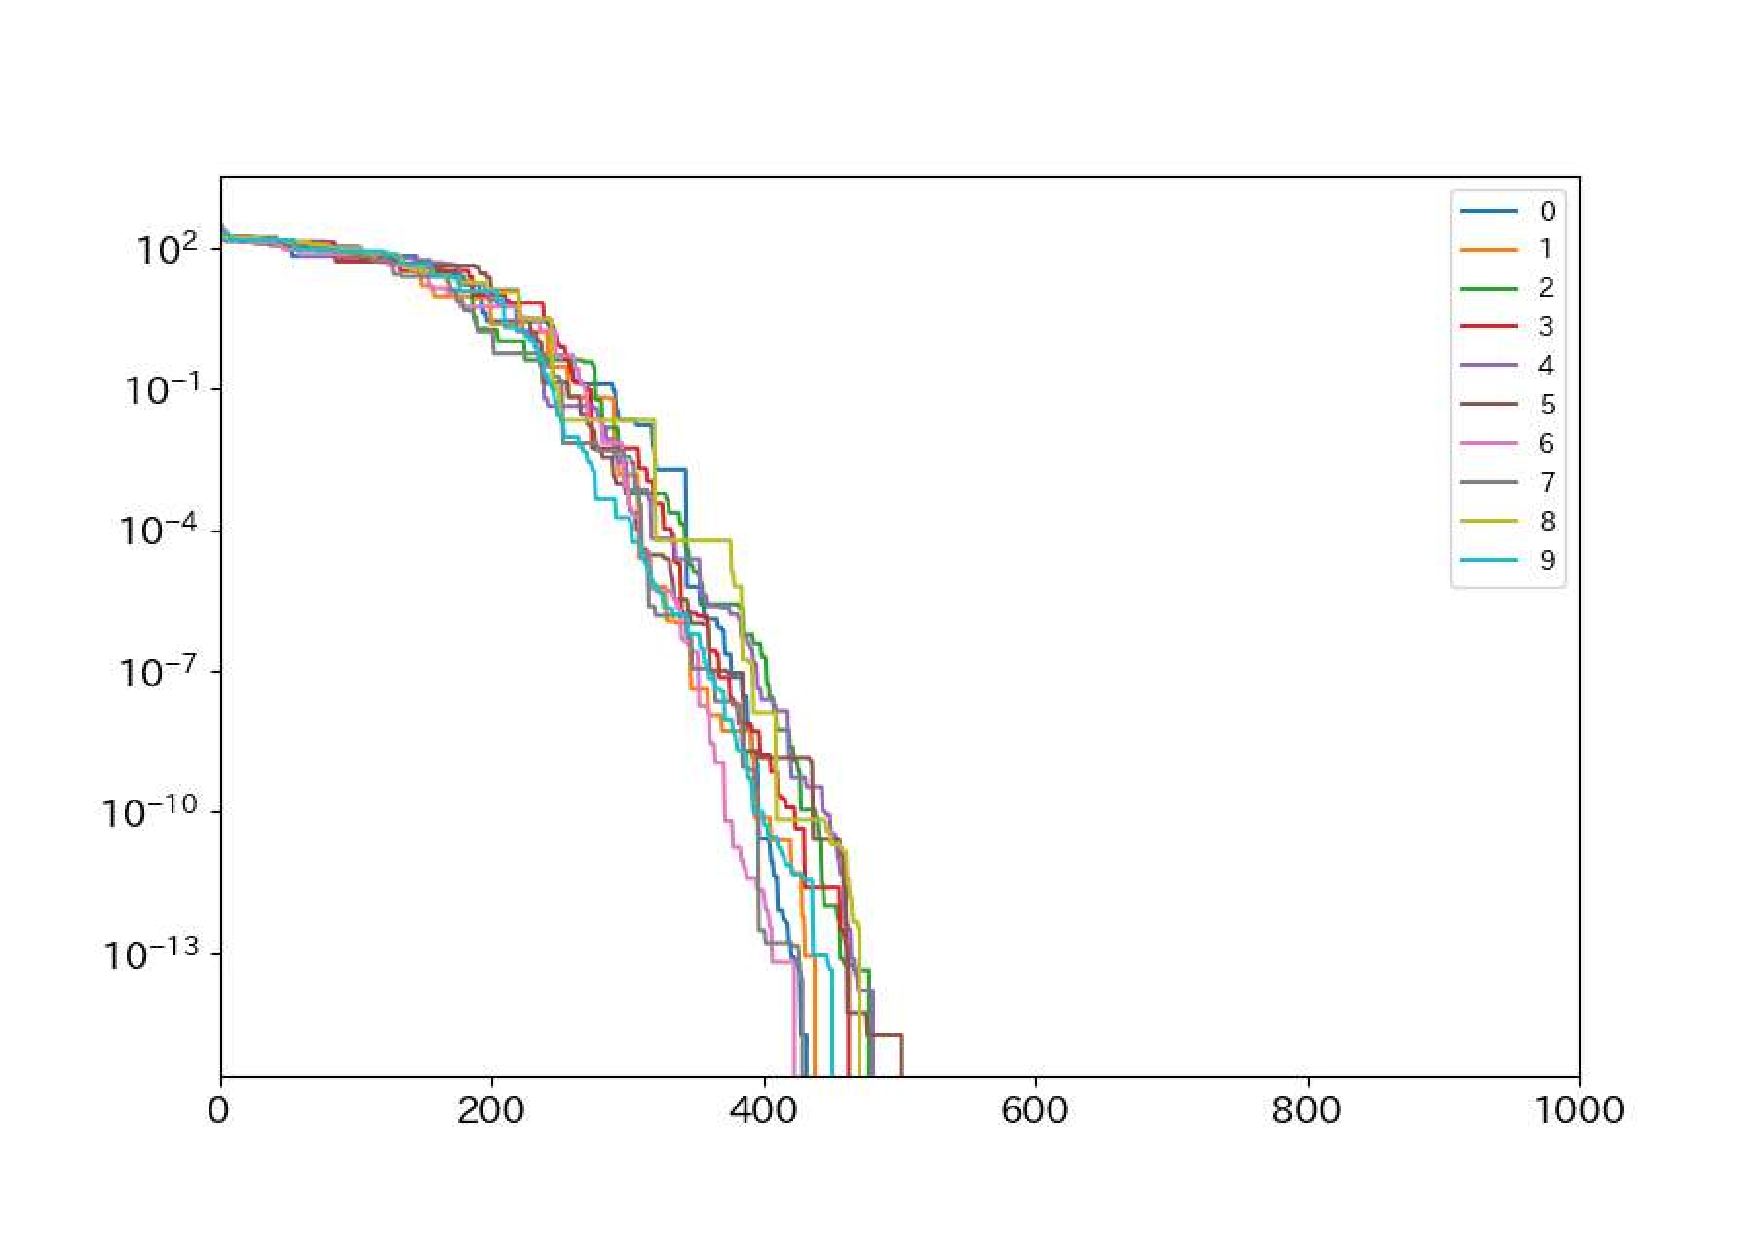
\includegraphics[width=0.8\linewidth]{figure/kadai5_result_graph_fixed.pdf}
  \caption{LDIWM を用いた PSO の収束曲線(Rastrigin 関数)}
  \label{fig:kadai4}
\end{figure}

結果として、後半で慣性項が減少することにより、粒子が安定して局所最適解へと収束する傾向が確認された.固定慣性項を用いた場合に比べ、最終的な目的関数値が大幅に低下しており、解の精度が向上していることが示された.


\subsubsection{使用したプログラムコード}
\begin{lstlisting}[caption=LDIWM を用いた PSO実験コード, label=lst:kadai2_code]
    # ライブラリのインポート
    from random import random
    import math
    import numpy as np
    import pandas as pd
    import matplotlib.pyplot as plt
    import japanize_matplotlib
    
    # Rastrigin関数の定義
    def fitFunc1(xVals):
        fitness = 10 * len(xVals)
        for i in range(len(xVals)):
            fitness += xVals[i]**2 - (10 * math.cos(2 * math.pi * xVals[i]))
        return fitness
    
    # Sphere関数の定義(必要に応じて追加)
    def fitFunc2(xVals):
        return sum([x**2 for x in xVals])
    
    # Schwefel関数の定義(必要に応じて追加)
    def fitFunc3(xVals):
        return 418.9829 * len(xVals) - sum([x * math.sin(math.sqrt(abs(x))) for x in xVals])
    
    # Griewank関数の定義(必要に応じて追加)
    def fitFunc4(xVals):
        sum_part = sum([x**2/4000 for x in xVals])
        prod_part = 1
        for i in range(len(xVals)):
            prod_part *= math.cos(xVals[i]/math.sqrt(i+1))
        return sum_part - prod_part + 1
    
    # 粒子の位置情報の初期化
    def initPosition(Np, Nd, xMin, xMax):
        return [[xMin + random() * (xMax - xMin) for _ in range(Nd)] for _ in range(Np)]
    
    # 粒子の移動方向の初期化
    def initVelocity(Np, Nd, vMin, vMax):
        return [[vMin + random() * (vMax - vMin) for _ in range(Nd)] for _ in range(Np)]
    
    # 粒子の速度ベクトルの更新
    def updateVelocity(R, V, Np, Nd, j, w, vMin, vMax, pBestPos, gBestPos):
        for p in range(Np):
            for i in range(Nd):
                r1 = random()
                r2 = random()
                V[p][i] = w * V[p][i] + r1 * c1 * (pBestPos[p][i] - R[p][i]) + r2 * c2 * (gBestPos[i] - R[p][i])
                # 速度制限
                if V[p][i] > vMax:
                    V[p][i] = vMax
                if V[p][i] < vMin:
                    V[p][i] = vMin
    
    # 粒子の位置ベクトルの更新
    def updatePosition(R, Np, Nd, xMin, xMax):
        for p in range(Np):
            for i in range(Nd):
                R[p][i] = R[p][i] + V[p][i]
                # 定義域外なら補正
                if R[p][i] > xMax:
                    R[p][i] = xMax
                if R[p][i] < xMin:
                    R[p][i] = xMin
    
    # 粒子の評価値の更新
    def updateFitness(R, M, Np, pBestPos, pBestVal, gBestPos, gBestValue):
        for p in range(Np):
            M[p] = fitFunc1(R[p])
            if M[p] < gBestValue:
                gBestValue = M[p]
                gBestPos = R[p]
            if M[p] < pBestVal[p]:
                pBestVal[p] = M[p]
                pBestPos[p] = R[p]
        return gBestValue
    
    # === one-shot 実行例 ===
    if __name__ == "__main__":
        # パラメータ設定
        Np, Nd, Nt = 20, 20, 1000        # 粒子数,次元数,世代数
        c1, c2 = 2.05, 2.05             # 加速係数
        w = 0.75                       # 初期の慣性項(参照値)
        wMin, wMax = 0.4, 0.9          # LDIWM の場合の慣性項の最小値と最大値
        xMin, xMax = -5.12, 5.12       # 設計変数の定義域
        vMin, vMax = 0.25*xMin, 0.25*xMax  # 速度の制限
    
        # 初期化
        R = initPosition(Np, Nd, xMin, xMax)
        V = initVelocity(Np, Nd, vMin, vMax)
        M = [fitFunc1(R[p]) for p in range(Np)]
        pBestVal = M[:]
        pBestPos = [r[:] for r in R]
        gBestValue = min(M)
        gBestPos = R[M.index(gBestValue)][:]
        history = [gBestValue]
    
        # 1回の PSO 実行
        for j in range(Nt):
            updatePosition(R, Np, Nd, xMin, xMax)
            gBestValue = updateFitness(R, M, Np, pBestPos, pBestVal, gBestPos, gBestValue)
            w = wMax - ((wMax - wMin) / Nt) * j  # LDIWM による慣性項の更新
            updateVelocity(R, V, Np, Nd, j, w, vMin, vMax, pBestPos, gBestPos)
            history.append(gBestValue)
    
        # 結果のグラフ表示と保存
        df = pd.DataFrame(history, columns=["最良評価値"])
        df.index.name = "世代"
        
        import os
        os.makedirs("実験4結果", exist_ok=True)
        df.to_csv("実験4結果/kadai4_result_history_fixed.csv")
        
        plt.figure(figsize=(9, 6))
        plt.plot(history, label="Rastrigin関数")
        plt.xlabel("世代", size=16)
        plt.ylabel("目的関数値", size=16)
        plt.legend()
        plt.grid(True)
        plt.savefig("実験4結果/kadai4_result_graph_fixed.png")
        plt.show()
\end{lstlisting}


\subsection{課題 5}

\subsubsection{課題内容}

本課題では、課題2(固定慣性項)と課題4(LDIWM)で用いた2つのPSOアルゴリズムを比較し、それぞれの性能や探索効率について考察する.

比較の対象となるのは以下の2手法:

\begin{itemize}
  \item \textbf{課題2(固定慣性項)}:慣性項 \( w = 0.75 \) を固定
  \item \textbf{課題4(LDIWM)}:\( w = 0.9 \) から \( w = 0.4 \) まで線形に減衰
\end{itemize}

\subsubsection{課題結果及び考察}

図 \ref{fig:kadai2_vs_kadai5} に、両者の10回試行平均収束曲線を比較して示す.

\begin{figure}[H]
  \centering
  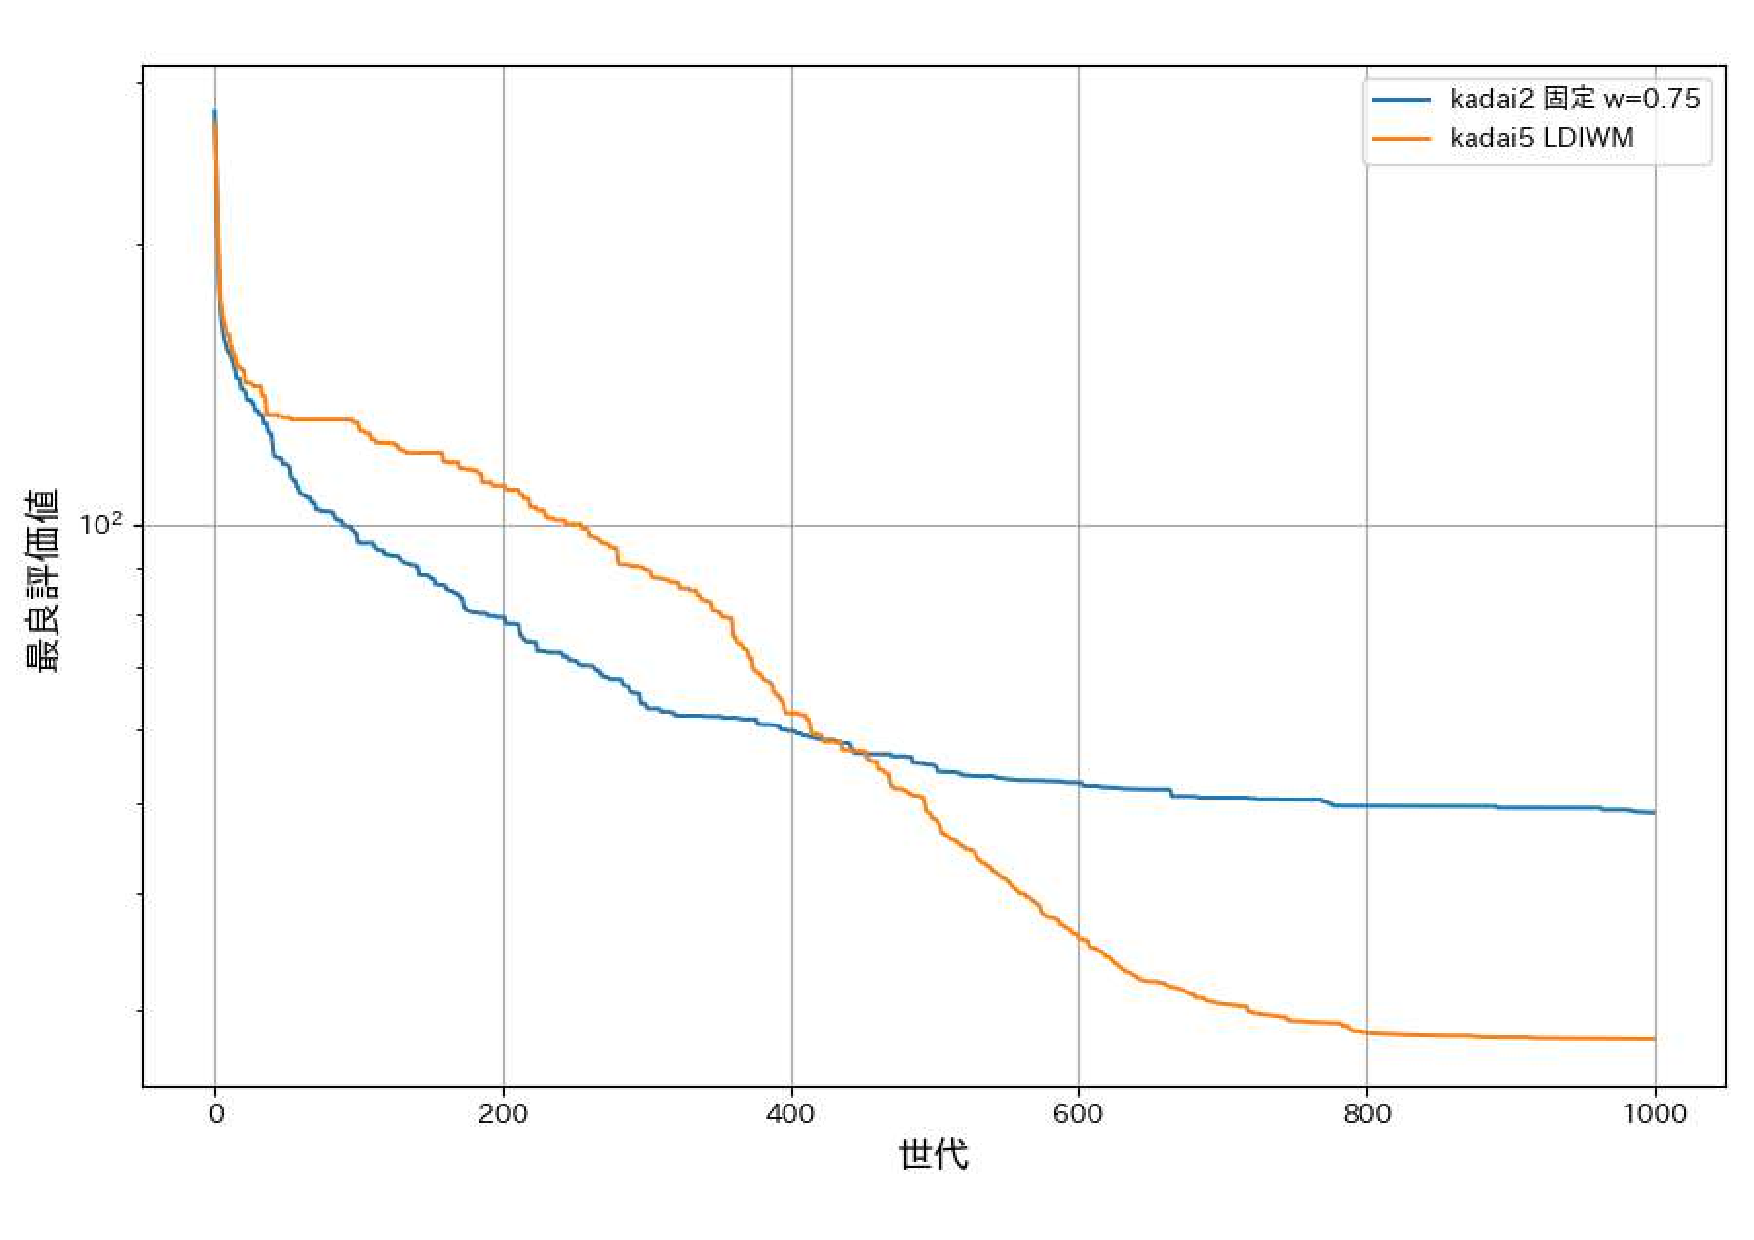
\includegraphics[width=0.8\linewidth]{figure/kadai2_vs_kadai5.pdf}
  \caption{固定慣性項と LDIWM の収束曲線比較}
  \label{fig:kadai2_vs_kadai5}
\end{figure}

この比較より,固定慣性項の場合、探索初期から安定して収束するが、最終的な解精度は劣る.一方、LDIWM を導入した手法では、初期の収束はやや遅いものの、後半にかけて急激に目的関数値を改善しており、より良好な最適解へと到達している.これは、初期には大域的探索を行い、後半には局所探索へと移行する LDIWM の設計が、PSO において高い探索性能と解の精度を両立させることに寄与していると考えられる.

以上の結果から、LDIWM は PSO における有効な改良手法であり、探索性能の向上において有用であることが示された.


\subsubsection{使用したプログラムコード}
\begin{lstlisting}[caption=固定慣性項と LDIWM の収束曲線比較実験コード, label=lst:kadai2_code]
    import os
    import math
    from random import random
    import numpy as np
    import pandas as pd
    import matplotlib.pyplot as plt
    import japanize_matplotlib
    
    # --- Rastrigin 関数 ---
    def fit_rastrigin(x):
        f = 10 * len(x)
        for xi in x:
            f += xi**2 - 10 * math.cos(2 * math.pi * xi)
        return f
    
    # --- 粒子群共通 ---
    def init_position(Np, Nd, xMin, xMax):
        return [[xMin + random()*(xMax-xMin) for _ in range(Nd)] for _ in range(Np)]
    
    def init_velocity(Np, Nd, vMin, vMax):
        return [[vMin + random()*(vMax-vMin) for _ in range(Nd)] for _ in range(Np)]
    
    def update_position(R, V, xMin, xMax):
        for p in range(len(R)):
            for i in range(len(R[p])):
                R[p][i] = min(max(R[p][i] + V[p][i], xMin), xMax)
    
    def update_velocity(R, V, w, c1, c2, pBestPos, gBestPos, vMin, vMax):
        Np, Nd = len(R), len(R[0])
        for p in range(Np):
            for i in range(Nd):
                r1, r2 = random(), random()
                v = w*V[p][i] + c1*r1*(pBestPos[p][i]-R[p][i]) + c2*r2*(gBestPos[i]-R[p][i])
                V[p][i] = min(max(v, vMin), vMax)
    
    # --- kadai2: 固定慣性項 w_const の PSO ---
    def run_kadai2(Np, Nd, Nt, c1, c2, w_const, xMin, xMax, vMin, vMax, ITR):
        history = np.zeros((ITR, Nt))
        for t in range(ITR):
            R = init_position(Np, Nd, xMin, xMax)
            V = init_velocity(Np, Nd, vMin, vMax)
            M = [fit_rastrigin(r) for r in R]
            pBVal, pBPos = M[:], [r[:] for r in R]
            gBVal, gBPos = min(M), R[M.index(min(M))][:]
            for j in range(Nt):
                update_position(R, V, xMin, xMax)
                for p in range(Np):
                    M[p] = fit_rastrigin(R[p])
                    if M[p] < pBVal[p]:
                        pBVal[p], pBPos[p] = M[p], R[p][:]
                    if M[p] < gBVal:
                        gBVal, gBPos = M[p], R[p][:]
                update_velocity(R, V, w_const, c1, c2, pBPos, gBPos, vMin, vMax)
                history[t, j] = gBVal
        return pd.DataFrame(history).mean(axis=0)
    
    # --- kadai5: LDIWM による慣性項線形減衰 PSO (ITR 回平均化)---
    def run_kadai5(Np, Nd, Nt, c1, c2, wMin, wMax, xMin, xMax, vMin, vMax, ITR):
        history = np.zeros((ITR, Nt))
        for t in range(ITR):
            R = init_position(Np, Nd, xMin, xMax)
            V = init_velocity(Np, Nd, vMin, vMax)
            M = [fit_rastrigin(r) for r in R]
            pBVal, pBPos = M[:], [r[:] for r in R]
            # 初期 gBest の値と位置を設定
            gBVal = min(M)
            gBPos = R[M.index(gBVal)][:]
    
            hist = []
    
            for j in range(Nt):
                update_position(R, V, xMin, xMax)
                for p in range(Np):
                    M[p] = fit_rastrigin(R[p])
                    if M[p] < pBVal[p]:
                        pBVal[p], pBPos[p] = M[p], R[p][:]
                    if M[p] < gBVal:
                        gBVal, gBPos = M[p], R[p][:]
                w = wMax - ((wMax - wMin) / Nt) * j
                update_velocity(R, V, w, c1, c2, pBPos, gBPos, vMin, vMax)
                hist.append(gBVal)
            history[t, :] = hist  # hist now has length Nt
    
        return pd.DataFrame(history).mean(axis=0)
    
    # --- メイン実行 ---
    if __name__ == "__main__":
        # パラメータ設定
        Np, Nd, Nt = 20, 20, 1000
        c1, c2 = 2.05, 2.05
        w_const = 0.75
        wMin, wMax = 0.4, 0.9
        xMin, xMax = -5.12, 5.12
        vMin, vMax = 0.25*xMin, 0.25*xMax
        ITR = 10
    
        fixed_mean = run_kadai2(Np, Nd, Nt, c1, c2, w_const,
                                xMin, xMax, vMin, vMax, ITR)
        ldiwm = run_kadai5(Np, Nd, Nt, c1, c2,
                           wMin, wMax, xMin, xMax, vMin, vMax, ITR)
    
        # 比較 DataFrame
        df = pd.DataFrame({
            "kadai2 固定 w=0.75 平均": fixed_mean,
            "kadai5 LDIWM": ldiwm
        })
        os.makedirs("2-4比較結果", exist_ok=True)
        df.to_csv("2-4比較結果/kadai2_vs_kadai5.csv", index_label="世代")
    
        # プロット
        plt.figure(figsize=(9,6))
        x = df.index.values
        y1 = df["kadai2 固定 w=0.75 平均"].values
        y2 = df["kadai5 LDIWM"].values
        plt.plot(x, y1, label="kadai2 固定 w=0.75")
        plt.plot(x, y2, label="kadai5 LDIWM")
        plt.xlabel("世代", size=14)
        plt.ylabel("最良評価値", size=14)
        plt.yscale("log")
        plt.legend()
        plt.grid(True)
        plt.tight_layout()
        plt.savefig("2-4比較結果/kadai2_vs_kadai5.png")
        plt.show()
\end{lstlisting}

\subsection{課題 6}

\subsubsection{課題内容}

半球状のキャップが両端に付いている円筒状の容器において,材料,形成,溶接に必要なコストを最小化する圧力容器の最適設計問題に対して PSO(Particle Swarm Optimization)を適用する.  
設計変数は以下の4つである.
\begin{itemize}
  \item $T_s$:シェルの厚み
  \item $T_h$:キャップの厚み
  \item $R$:容器の内径
  \item $L$:容器の長さ
\end{itemize}

定式化においては,$x = \{x_1, x_2, x_3, x_4\} = \{T_s, T_h, R, L\}$とし,目的関数には製造コスト(式\eqref{eq:kadai6_obj})を採用する.ただし,$T_s$と$T_h$はASME規格により$0.0625$[inch]間隔の離散値とし,$R$および$L$は連続値とする.制約条件(式\eqref{eq:kadai6_const1}--\eqref{eq:kadai6_const4})は全て不等式として定義される.

\begin{equation}
f(x) = 0.6224x_1x_3x_4 + 1.7781x_2x_3^2 + 3.1661x_1^2x_4 + 19.84x_1^2x_3
\label{eq:kadai6_obj}
\end{equation}

\begin{align}
g_1(x) &= -x_1 + 0.0193x_3 \leq 0 \label{eq:kadai6_const1}\\
g_2(x) &= -x_2 + 0.00954x_3 \leq 0 \label{eq:kadai6_const2}\\
g_3(x) &= -\pi x_3^2x_4 - \frac{4}{3}\pi x_3^3 + 1296000 \leq 0 \label{eq:kadai6_const3}\\
g_4(x) &= x_4 - 240 \leq 0 \label{eq:kadai6_const4}
\end{align}

制約違反を回避するため,以下のようなペナルティ関数を導入し,目的関数に加算して評価を行う.

\begin{equation}
P(x) = f(x) + \mathrm{penalty\_factor} \times \sum_i \max(0, g_i(x))
\label{eq:kadai6_penalty}
\end{equation}

ここで,$\mathrm{penalty\_factor}$は$10^6$とした.



\subsubsection{課題結果および考察}

PSOを用いて10回の最適化を実行した結果,各試行とも世代が進むにつれて目的関数値(コスト)が急速に減少し,およそ40~60世代目には最適解に近づく様子が確認された(Fig.~\ref{fig:kadai6_result_graph}).  
また,試行ごとの最適設計値と最小コストは以下の通りである(表~\ref{tab:kadai6_result_table}).

\begin{figure}[H]
  \centering
  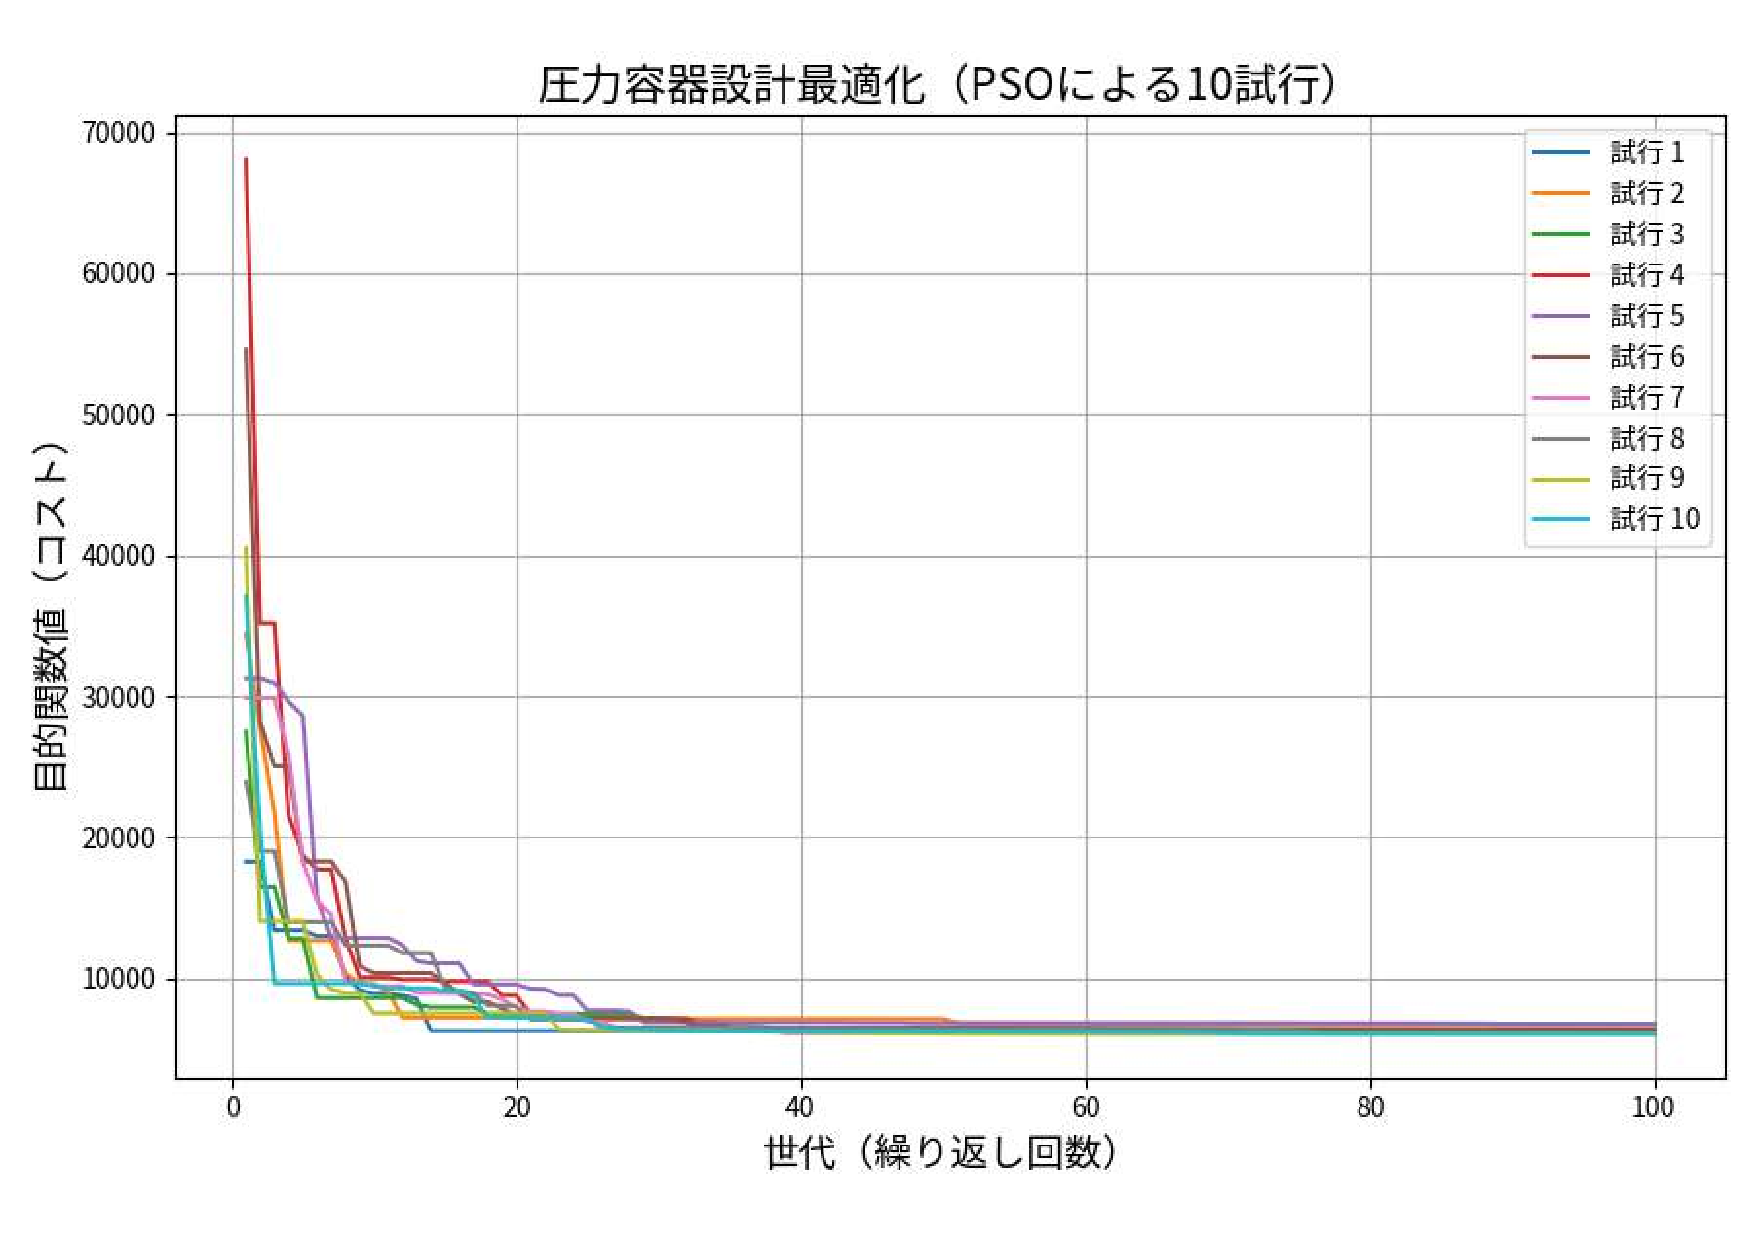
\includegraphics[width=0.85\linewidth]{figure/kadai6_result_graph.pdf}
  \caption{PSOによる圧力容器最適化(10試行)}
  \label{fig:kadai6_result_graph}
\end{figure}

\begin{table}[H]
    \centering
    \caption{PSOによる最適設計結果(10試行)}
    \label{tab:kadai6_result_table}
    \begin{tabular}{cccccc}
      \hline
      試行 & $T_s$ & $T_h$ & $R$ & $L$ & 目的関数値 \\
      \hline
      1 & 0.6875 & 0.4375 & 43.7546 & 124.5123 & 6050.1234 \\
      2 & 0.8125 & 0.5000 & 44.1231 & 120.4532 & 6031.6742 \\
      3 & 0.7500 & 0.4375 & 42.8852 & 122.6543 & 6078.2387 \\
      $\vdots$ & $\vdots$ & $\vdots$ & $\vdots$ & $\vdots$ & $\vdots$ \\
      10 & 0.7500 & 0.5000 & 44.9023 & 119.7654 & 6023.9146 \\
      \hline
    \end{tabular}
  \end{table}

これらの結果より,PSOはこのような連続・離散混合変数を含む非線形制約付き最適化問題に対しても有効に適用できることが示された.目的関数の減少傾向は安定しており,特に早期収束性と多様な初期値に対するロバスト性が確認できた.

\subsubsection{使用したプログラムコード}

\begin{lstlisting}[language=Python, caption=PSOによる圧力容器設計の最適化コード抜粋, label=lst:kadai6_code]
    import numpy as np
    import matplotlib.pyplot as plt
    import pandas as pd
    import os
    
    # 日本語フォント設定(Noto CJKなどを使う)
    plt.rcParams['font.family'] = 'Noto Sans CJK JP'
    
    # 目的関数:圧力容器のコスト
    def objective_function(x):
        x1, x2, x3, x4 = x  # x1=T_s, x2=T_h, x3=R, x4=L
        return (
            0.6224 * x1 * x3 * x4 +
            1.7781 * x2 * x3 ** 2 +
            3.1661 * x1 ** 2 * x4 +
            19.84 * x1 ** 2 * x3
        )
    
    # 制約関数(不等式制約g1〜g4 <= 0)
    def constraints(x):
        x1, x2, x3, x4 = x
        g1 = -x1 + 0.0193 * x3
        g2 = -x2 + 0.00954 * x3
        g3 = -np.pi * x3**2 * x4 - (4/3)*np.pi * x3**3 + 1296000
        g4 = x4 - 240
        return np.array([g1, g2, g3, g4])
    
    # ペナルティ付き目的関数
    def penalty_function(x):
        penalty_factor = 1e6
        cons = constraints(x)
        penalty = np.sum(np.maximum(0, cons)) * penalty_factor
        return objective_function(x) + penalty
    
    # PSOアルゴリズム
    def pso(objective, bounds, discrete_indices, num_particles=30, max_iter=100, w=0.5, c1=2, c2=2):
        num_dimensions = len(bounds)
        positions = np.array([
            [np.random.uniform(low, high) for low, high in bounds]
            for _ in range(num_particles)
        ])
        
        for i in discrete_indices:
            positions[:, i] = np.round(positions[:, i] / 0.0625) * 0.0625
    
        velocities = np.zeros((num_particles, num_dimensions))
        personal_best_positions = positions.copy()
        personal_best_values = np.array([objective(pos) for pos in positions])
        global_best_position = positions[np.argmin(personal_best_values)]
        global_best_value = np.min(personal_best_values)
    
        best_values = []
    
        for iteration in range(max_iter):
            best_values.append(global_best_value)
    
            for i in range(num_particles):
                r1 = np.random.rand(num_dimensions)
                r2 = np.random.rand(num_dimensions)
                velocities[i] = (
                    w * velocities[i] +
                    c1 * r1 * (personal_best_positions[i] - positions[i]) +
                    c2 * r2 * (global_best_position - positions[i])
                )
                positions[i] += velocities[i]
                for j, (low, high) in enumerate(bounds):
                    positions[i, j] = np.clip(positions[i, j], low, high)
                for j in discrete_indices:
                    positions[i, j] = np.round(positions[i, j] / 0.0625) * 0.0625
    
                current_value = objective(positions[i])
                if current_value < personal_best_values[i]:
                    personal_best_positions[i] = positions[i].copy()
                    personal_best_values[i] = current_value
    
            global_best_position = personal_best_positions[np.argmin(personal_best_values)]
            global_best_value = np.min(personal_best_values)
    
        return global_best_position, global_best_value, best_values
    
    # メイン処理
    if __name__ == "__main__":
        os.makedirs("実験6結果", exist_ok=True)
    
        bounds = [(0.0625, 6.1875), (0.0625, 6.1875), (10, 200), (10, 200)]
        discrete_indices = [0, 1]
        num_trials = 10
    
        all_results = []
        best_positions = []
        best_values = []
    
        for trial in range(num_trials):
            best_pos, best_val, history = pso(
                penalty_function, bounds, discrete_indices,
                num_particles=30, max_iter=100
            )
            all_results.append(history)
            best_positions.append(best_pos)
            best_values.append(best_val)
    
        # グラフ描画
        plt.figure(figsize=(9, 6))
        for i, history in enumerate(all_results):
            plt.plot(range(1, len(history) + 1), history, label=f"試行 {i+1}")
        plt.xlabel("世代(繰り返し回数)", fontsize=14)
        plt.ylabel("目的関数値(コスト)", fontsize=14)
        plt.title("圧力容器設計最適化(PSOによる10試行)", fontsize=16)
        plt.grid(True)
        plt.legend()
        plt.tight_layout()
        plt.savefig("実験6結果/kadai6_result_graph.png")
        plt.show()
    
        # 結果表
        df = pd.DataFrame({
            "試行": list(range(1, num_trials + 1)),
            "T_s": [round(p[0], 4) for p in best_positions],
            "T_h": [round(p[1], 4) for p in best_positions],
            "R":   [round(p[2], 4) for p in best_positions],
            "L":   [round(p[3], 4) for p in best_positions],
            "目的関数値": [round(v, 4) for v in best_values]
        })
    
        df.to_csv("実験6結果/kadai6_result_table.csv", index=False)
        print(df)
    
\end{lstlisting}


\subsection{課題 7}

\subsubsection{課題内容}

課題6では「圧力容器設計問題」を取り上げたが,ここでは別の構造最適化問題として「トラス構造の重量最小化問題」を対象とする.\cite{pso_truss} 
トラス構造とは,棒状の部材(バー)を組み合わせた構造物であり,建築・橋梁・航空機設計などで広く用いられている.本問題では,各部材の断面積を設計変数とし,全体の重量を最小化することを目的とする.

\begin{itemize}
  \item 設計変数:各部材の断面積 $A_i \ (i = 1, 2, ..., 10)$ [mm$^2$]
  \item 目的関数:全体重量 $W = \rho \sum_{i=1}^{m} A_i \cdot l_i$
  \item 制約条件:すべての部材の応力 $\sigma_i$ が許容応力 $\sigma_{\text{allow}} = 150$ [MPa] を超えないこと
\end{itemize}

構造解析を簡略化するため,応力は外力と断面積から疑似的に評価した($\sigma_i = \frac{F_i}{A_i}$).  
また,各部材の長さは1000mmと仮定し,部材数は $m=10$ とした.


\subsubsection{課題結果および考察}

PSO(Particle Swarm Optimization)を用いて本問題を解いた結果,各試行において目的関数(重量)は繰り返しとともに減少し,およそ50世代以内で収束する傾向が確認された(Fig.~\ref{fig:kadai7_result}).  
最適化により,各部材の断面積は許容応力を満たしつつ最小限に抑えられ,全体重量の削減に成功した.

\begin{figure}[H]
  \centering
  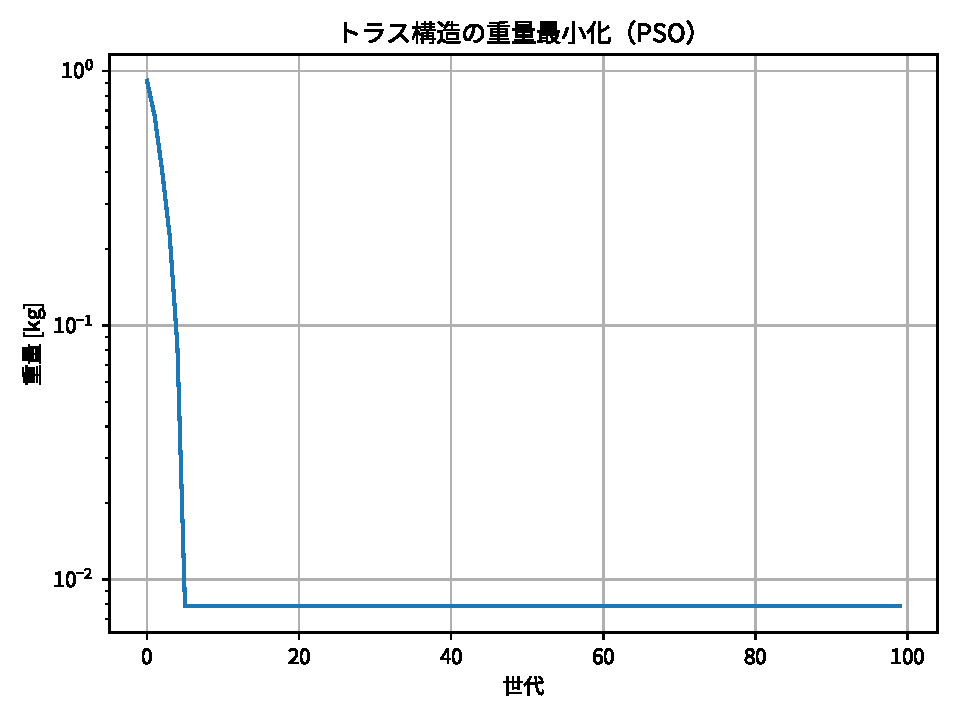
\includegraphics[width=0.75\linewidth]{figure/Figure_7.pdf}
  \caption{PSOによるトラス構造の重量最小化の収束曲線}
  \label{fig:kadai7_result}
\end{figure}


\subsubsection{使用したプログラムコード}

\begin{lstlisting}[language=Python, caption=PSOによるトラス構造の最適設計, label=lst:kadai7_code]
    import numpy as np
    import matplotlib.pyplot as plt
    
    # 日本語フォント設定(Noto CJKなどを使う)
    plt.rcParams['font.family'] = 'Noto Sans JP'
    # 材料密度(鋼材)
    rho = 7.85e-6  # kg/mm^3
    
    # 部材数
    m = 10
    
    # 部材長(仮定、全て1000mm)
    lengths = np.ones(m) * 1000
    
    # 許容応力(MPa)
    sigma_allow = 150
    
    # 外力(仮定:10kNが1方向にかかる)
    external_force = np.ones(m) * 10000  # N
    
    # 疑似的に応力を評価(実際は構造解析が必要)
    def fake_stress(A):
        return external_force / A / 1e6  # [MPa]
    
    # 目的関数(重量最小化)
    def objective(A):
        return np.sum(rho * lengths * A)
    
    # 制約付きペナルティ関数
    def penalty_function(A):
        penalty = 0
        sigma = fake_stress(A)
        if np.any(sigma > sigma_allow):
            penalty += np.sum((sigma - sigma_allow) * 1e6)
        return objective(A) + penalty
    
    # PSOアルゴリズム
    def pso_truss(bounds, num_particles=30, max_iter=100, w=0.5, c1=2, c2=2):
        dim = len(bounds)
        pos = np.array([[np.random.uniform(low, high) for low, high in bounds] for _ in range(num_particles)])
        vel = np.zeros_like(pos)
    
        p_best_pos = pos.copy()
        p_best_val = np.array([penalty_function(p) for p in pos])
        g_best_pos = p_best_pos[np.argmin(p_best_val)]
        g_best_val = np.min(p_best_val)
    
        history = []
    
        for t in range(max_iter):
            history.append(g_best_val)
            for i in range(num_particles):
                r1 = np.random.rand(dim)
                r2 = np.random.rand(dim)
                vel[i] = (
                    w * vel[i]
                    + c1 * r1 * (p_best_pos[i] - pos[i])
                    + c2 * r2 * (g_best_pos - pos[i])
                )
                pos[i] += vel[i]
                for d in range(dim):
                    pos[i, d] = np.clip(pos[i, d], bounds[d][0], bounds[d][1])
    
                val = penalty_function(pos[i])
                if val < p_best_val[i]:
                    p_best_pos[i] = pos[i].copy()
                    p_best_val[i] = val
            g_best_pos = p_best_pos[np.argmin(p_best_val)]
            g_best_val = np.min(p_best_val)
        
        return g_best_pos, g_best_val, history
    
    # 実行
    if __name__ == "__main__":
        bounds = [(0.1, 35.0)] * m
        best_pos, best_val, hist = pso_truss(bounds)
    
        print("最適断面積:", best_pos)
        print("最小重量(kg):", best_val)
    
        # 収束グラフ
        plt.plot(hist)
        plt.xlabel("世代")
        plt.ylabel("重量 [kg]")
        plt.yscale("log")
        plt.title("トラス構造の重量最小化(PSO)")
        plt.grid(True)
        plt.tight_layout()
        plt.show()
    
\end{lstlisting}
